\cappar En esta ocasión hemos tenido la oportunidad que el empleado de
Saema Luis Arantes Lemos de Azevedo nos visite en España y hemos
tenido el placer de conversar con él.  Os contamos algunas de nuestras
conversaciones que deseamos compartir con todos vosotros. ¡Gracias
Luis por tu visita!
\vspace{2cm}

{\bf Luis hablanos de tus orígenes.}


\vspace{10pt}

Nací en Luanda. Mi padre es de la región de Bengo y mi madre de
Luanda. Se conocieron en Luanda y se casaron. Su unión permitió tener
7 hijos, cinco chicas y dos chicos. Somos una familia muy unida y
aunque ya cada uno tiene su vida cada fin de semana hacemos por vernos
todos y compartir.

\vspace{10pt}

{\bf ¿Cómo viviste la guerra civil en tu país?}

\vspace{10pt}

Yo viví en Luanda por esos años y allí no fue tan brutal la guerra
pero por supuesto fue duro ver como la gente de tu país se desmorona y
se funde en la destrucción. Por suerte ahora el país está creciendo y
el espíritu de la gente es el de autosuperación y crecimiento
constante formándose siempre que tiene oportunidad para poder ``subir
de vida''.

\vspace{10pt}

{\bf Tu formación Luis, ¿puedes resumírnosla?}

\vspace{10pt}

Por supuesto. Yo estudié en el Instituto Medio Insdustrial de Luanda,
la especialización de Química. Después de ello viví una bella
experiencia trabajando en la enseñanza. Fui profesor de escuela por
unos años y me encantó ver que lo que uno enseña sirve para otros. Fue
muy gratificante. Después comencé a trabajar en Saema y ya son 8 años
colaborando con ellos. En Saema me dedico a la gestión administrativa,
control de salarios, control de horarios entre otras cosas. Primero
comencé trabajando en Cuanza Norte y después de tres años me transladé
a Luanda donde estoy actualmente.

\vspace{10pt}

{\bf ¿Cómo ve el trabajo que hace Saema?}

\vspace{10pt}

Muy fructífero. Mi país está en crecimiento y son muchos los lugares
que se encuentran sin agua, sin luz sin atención médica. Saema
aporta un granito de arena más para realizar el cambio que las
autoridades van consiguiendo poco a poco y es que cada angolano pueda
acceder a los servicios mínimos: luz, agua y medicina. A pesar de
todas las dificultaddes que tiene el angolano, es una persona que se
esfuerza, que trabaja y que desea alegremente un futuro mejor.
\vspace{10pt}

{\bf ¿Le gusta viajar?}

\vspace{10pt}

Sí. Antes de venir a este viaje a España,  había viajado a países
alrededor de Ángola. Esta es mi primera experiencia en Europa. Me
encanta viajar porque me encanta ver como cada gente tiene una
percepción del mundo, como cada gente tiene experiencias distintas de
trabajo, ver distintos ambientes. Todas las experiencias me hacen ser una
persona más abierta. Me gusta mucho viajar.

\vspace{10pt}

{\bf ¿Cúal es tu autor favorito?}

\vspace{10pt}

Uanhenga Xitu, él me marcó desde mi adolescencia y es un referente para mí.

\vspace{10pt}

{\bf Siempre pedimos a nuestros entrevistados que manden un
  mensaje a su pueblo. ¿Qué mensaje les manda usted, Luis?}

\vspace{10pt}

Tengan esperanza, el futuro va a ser mejor. 


\vspace{10pt}

{\bf Gracias Luis. Te deseamos lo mejor y te deseamos una \textcolor{red}{feliz
  boda} que parece te casas pronto. Suerte y, \textcolor{red}{¡vivan los novios!}

  \begin{figurebox}
    \vspace{20pt}
    \centering
    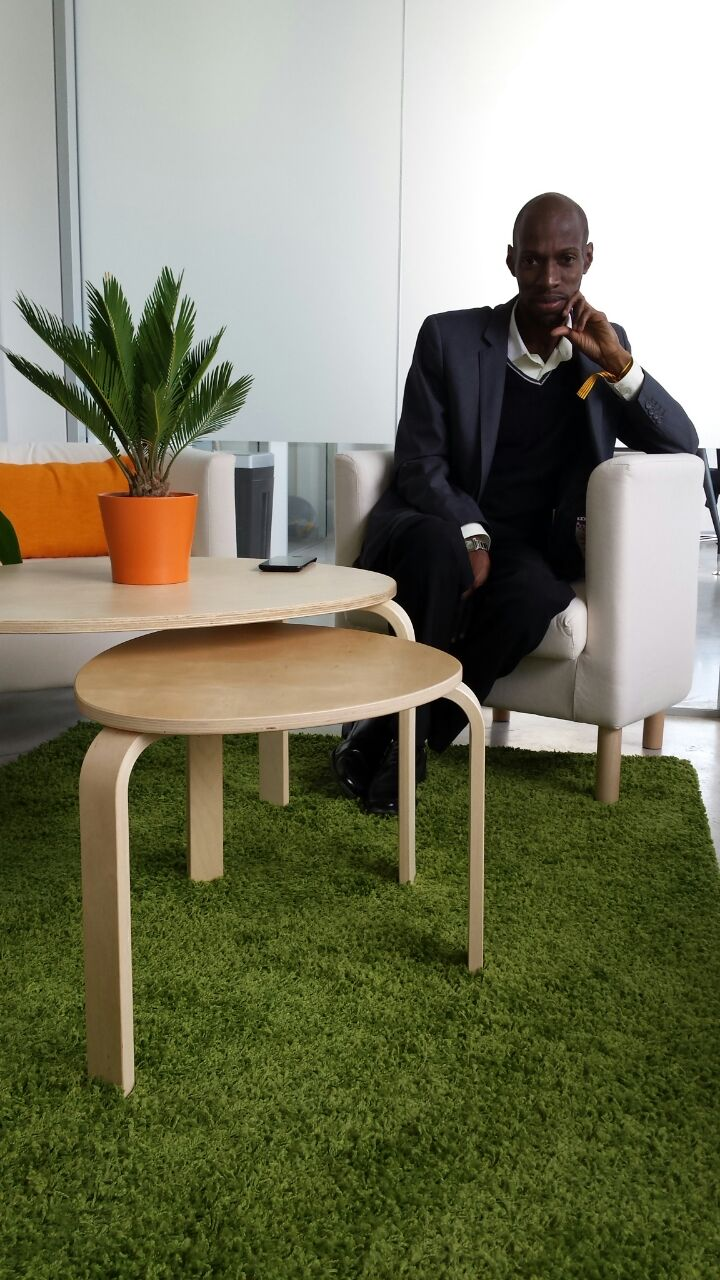
\includegraphics[scale=0.3]{luis.jpg}

     Luis Arantes Lemos de Azevedo\\
    {\sl Coordinador Administración de Saema}
    \vspace{20pt}
  \end{figurebox}

\newpage

%%% Local Variables: 
%%% mode: latex
%%% TeX-master: "solucionenaccion"
%%% End: 



